\section{\name Approach Overview}
\label{sec:approach}


\begin{figure}[t]
\centering
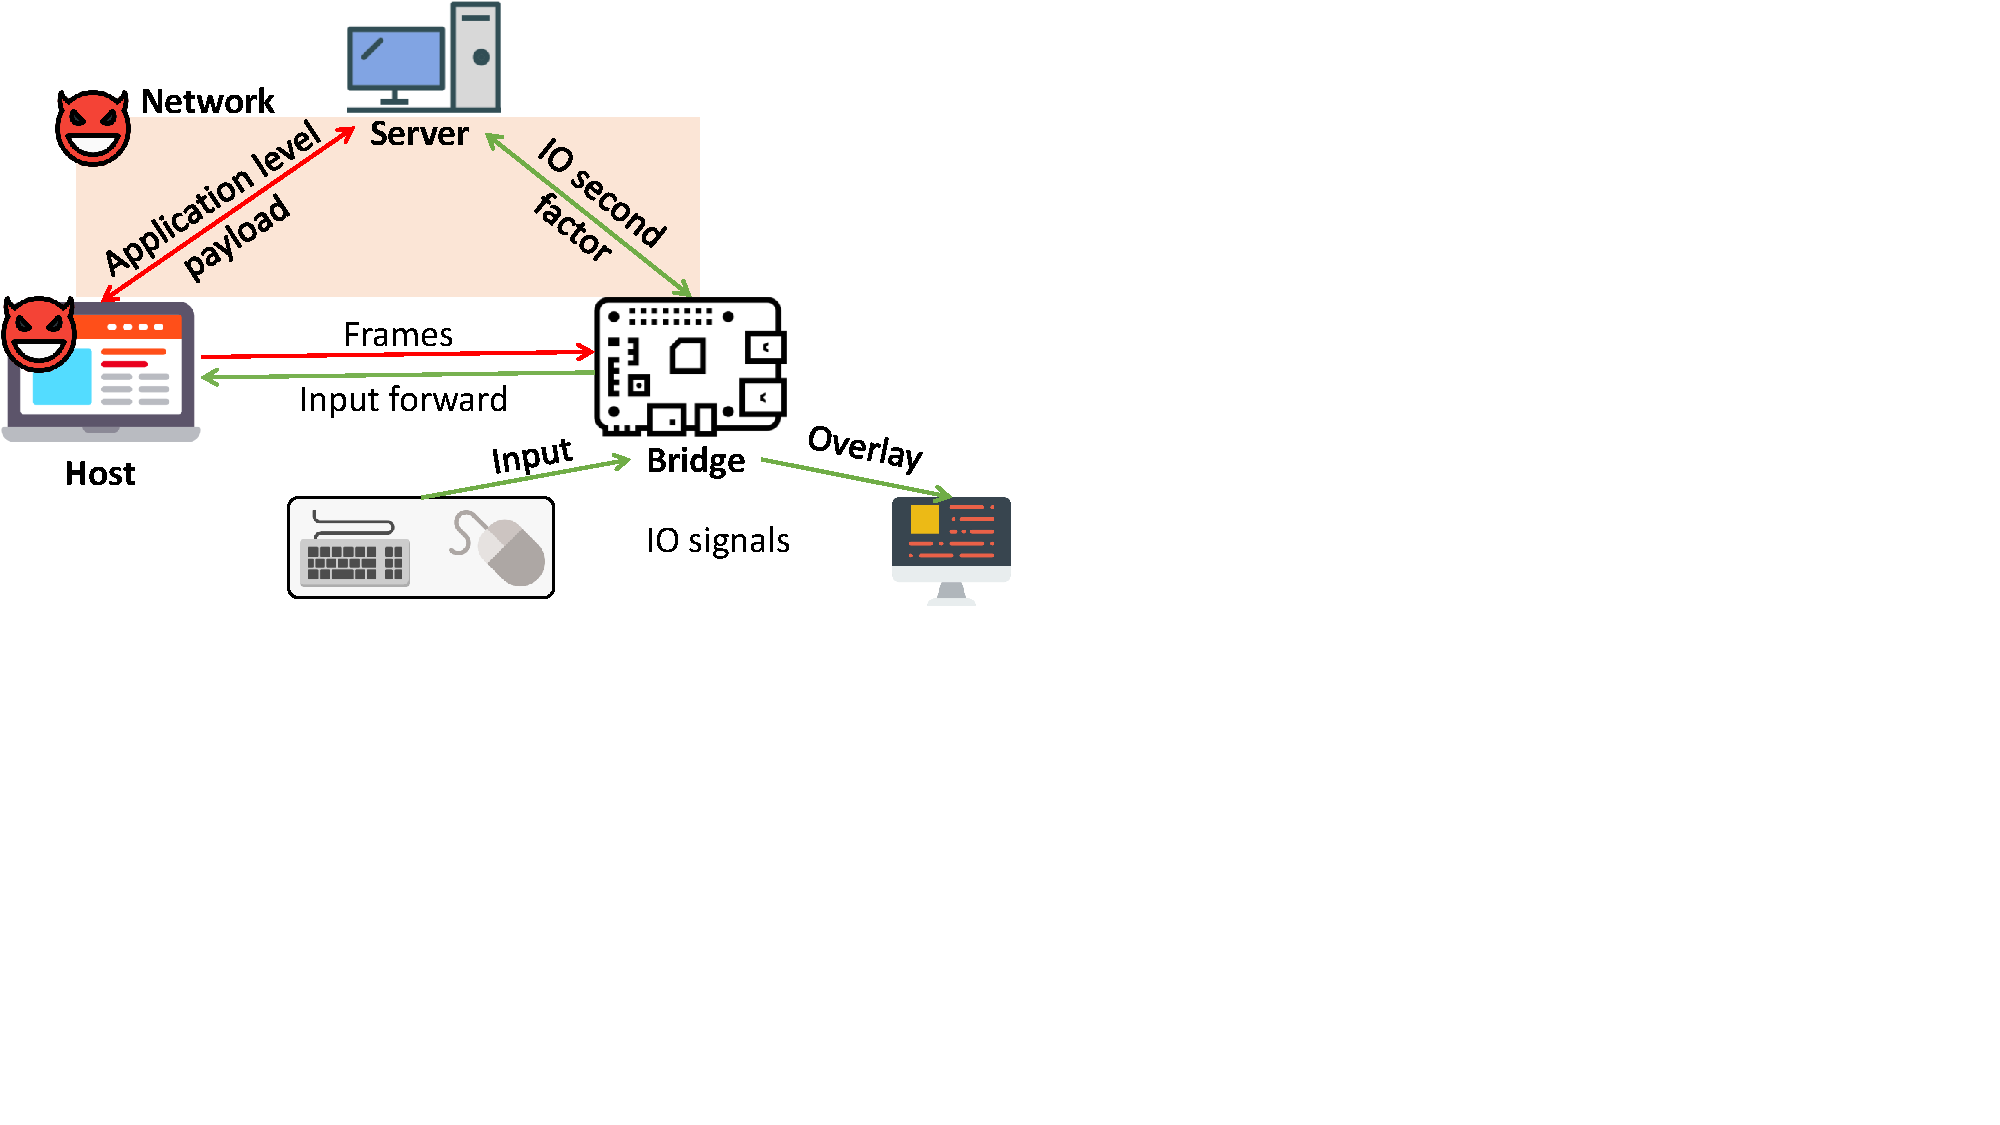
\includegraphics[trim={0 8.5cm 17cm 0}, clip, width=0.85\linewidth]{approachOverview.pdf}
\caption{\textbf{High-level approach overview of our solution.}  The \device connects the IO devices and the attacker-controlled host. We also assume that the network is also attacker-controlled.}
\spacesave
\label{fig:approachOverview}
\centering
\end{figure}


In this section, we present an overview of \name: our proposed solution. \name provides a trusted path between the user IO device and the remote server by utilizing a trusted embedded device (our approach fall into the category B1 in Figure~\ref{fig:relatedWorksTree}) as a mediator between all the IO devices and the untrusted host. We call this device: \device. The approach, on the high-level, uses the concept of the \emph{bump in the wire}~\cite{McCPerRei2006} to provide integrity and confidentiality to the user IO actions.  %The server also adds a small JavaScript snippet that allows the \device and the remote server to communicate. This eliminates any need for additional hardware/software aids.

We first define the system and attacker model, then outline the challenges and the brief outline of our proposed solution.

%Given the problem statement discussed in Section~\ref{sec:problemStatement}, we first define the attacker model we consider in our proposed system.


\subsection{System and Attacker Model}
\label{sec:approach:systemAttackerModel}

We consider a system model where the user wants to sends the input to a safety-critical remote end-system. The model is depicted in Figure~\ref{fig:approachOverview} that shows the untrusted host, remote server and the user IO devices. 

We assume that the attacker controls the host system completely (OS, installed applications and hardware). The attacker also controls the network. %We assume that the attacker is a probabilistic polynomial time (PPT) algorithm that can not break crypto. 
Figure~\ref{fig:approachOverview} shows the components of the system that are controlled by the attacker, i.e., the host and the network communication channel between the host and the remote server.

We only assume that the monitor, keyboard, mouse (in a word all the IO devices that we need to protect from the malicious host) and the \device are trusted.
%which is not unrealistic. The monitor, keyboard, and mouse have hardly any complex hardware. The TCB is very small.

The \device works as a mediator between all the IO devices and the host. Note that the \device has no network capability to communicate with the server, rather it relies on the host and use it as an untrusted transport. We also assume that the \device comes with some embedded certificates and keys that allow the \device to verify the signatures signed by the server and sign statements such as the user input. We can assume that the \device is issused by a service provider who also runs the remote server.

\myparagraph{Attacker's capability} As the host is attacker-controlled, it can intercept, drop or modify the user IO data to and from the remote server.On top of it, the host can launch complex UI-based attacks. Such includes spawning multiple mouse pointer to trick the user into following the wrong mouse pointer, changing the layout of the UI elements to trick the user into providing sensitive data, tricking the user into moving the mouse to the wrong location and click there, manipulate input data, etc.

\iffalse
\begin{figure}[t]
\centering
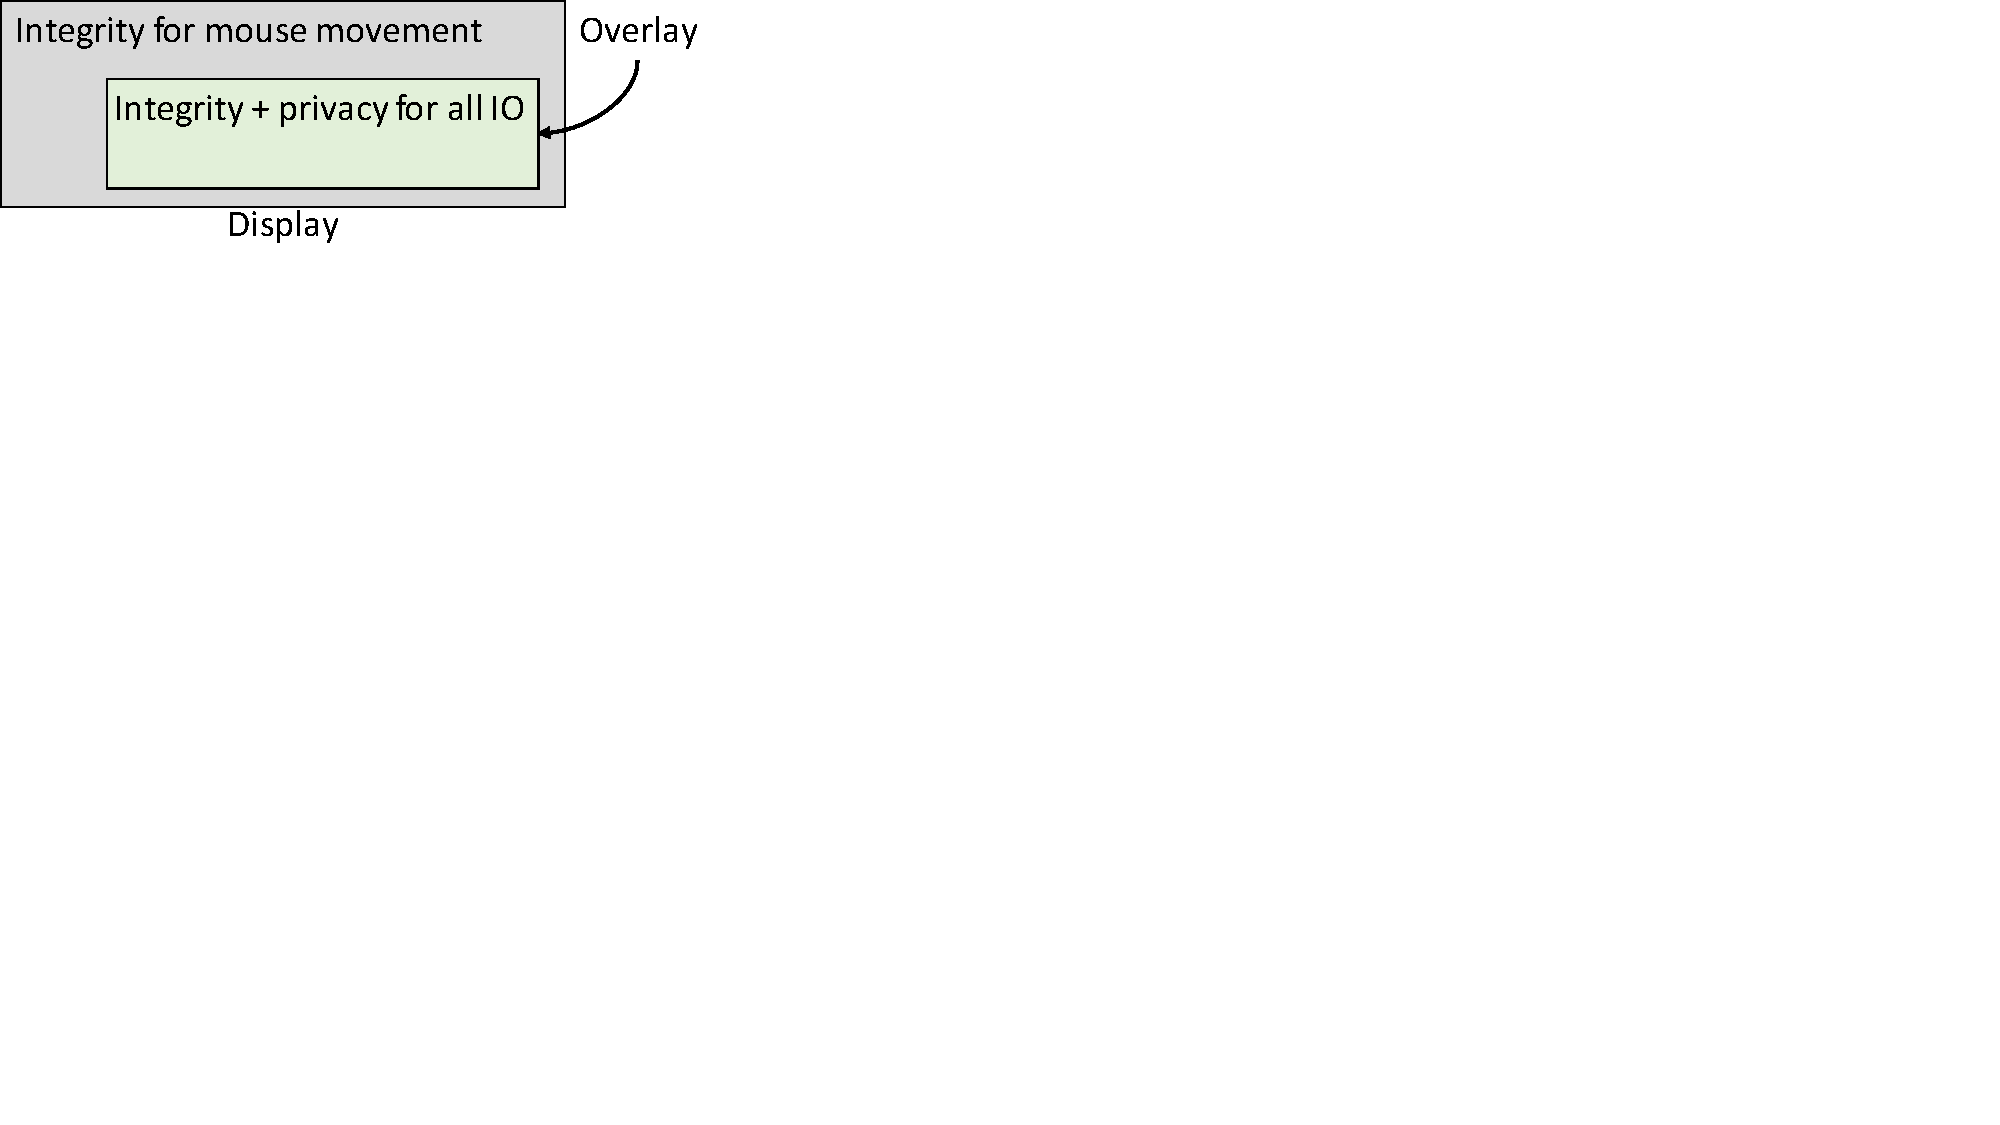
\includegraphics[trim={0 13cm 21.7cm 0}, clip, width=0.65\linewidth]{screenPartition.pdf}
\caption{\textbf{\device's pointer tracking, pointer \& UI overlay, and security properties.} Our proposed method provides two layers of protection for IO to the user. 1. In all the parts of the screen, the \device provide pointer integrity (the gray part). 2. The green part of the screen where the \device overlays on the HDMI stream where the \device provide integrity and privacy (privacy is dependent on the application requirements) for the IO.}
\spacesave
\label{fig:screenPartition}
\centering
\end{figure}
\fi


\subsection{Strawman Solutions}
\label{sec:approach:strawman}

Here we provide some strawman solutions and discuss the drawbacks of them.

\subsubsection{\bfseries Strawman solution I}
\label{sec:approach:strawman:1}

The first strawman solution is to use an external trusted device that is physically isolated from the attacker-controlled host. The external device runs a full operating system with a browser. Even though this approach works as the trust assumption dictates that the external device is trusted, but the security point of view, this approach does not provide any additional security - the external device as the same attack surface as the untrusted host due to its huge TCB.

\subsubsection{\bfseries Strawman solution II}
\label{sec:approach:strawman:2}

The second strawman solution is to use a trusted external device that contains a small program that signs all the user input and sends the signed input to the remote server. The device works as the second factor for input integrity as the remote server can verify if the signed input matched with the user input that is sent by the browser running on the untrusted host. IntegriKey~\cite{IntegriKey} provides such a solution that uses \webusb to send the signed input to the remote server. However, as the external device is completely oblivious to the display information that the untrusted host renders, it is vulnerable to a sophisticated UI manipulation attack. One such example could be, user's correct input is $100$ that she typed on a text box. However the host shows her $10$, thinking that she mistyped, the user types another $0$ that makes the recorded input from the user $1000$. This attack violates input integrity as the host can now submit $1000$ to the remote server as the external trusted device also signs $1000$ as the correct input received from the user.  

\subsubsection{\bfseries Strawman solution III}
\label{sec:approach:strawman:3}

\begin{figure}[t]
\centering
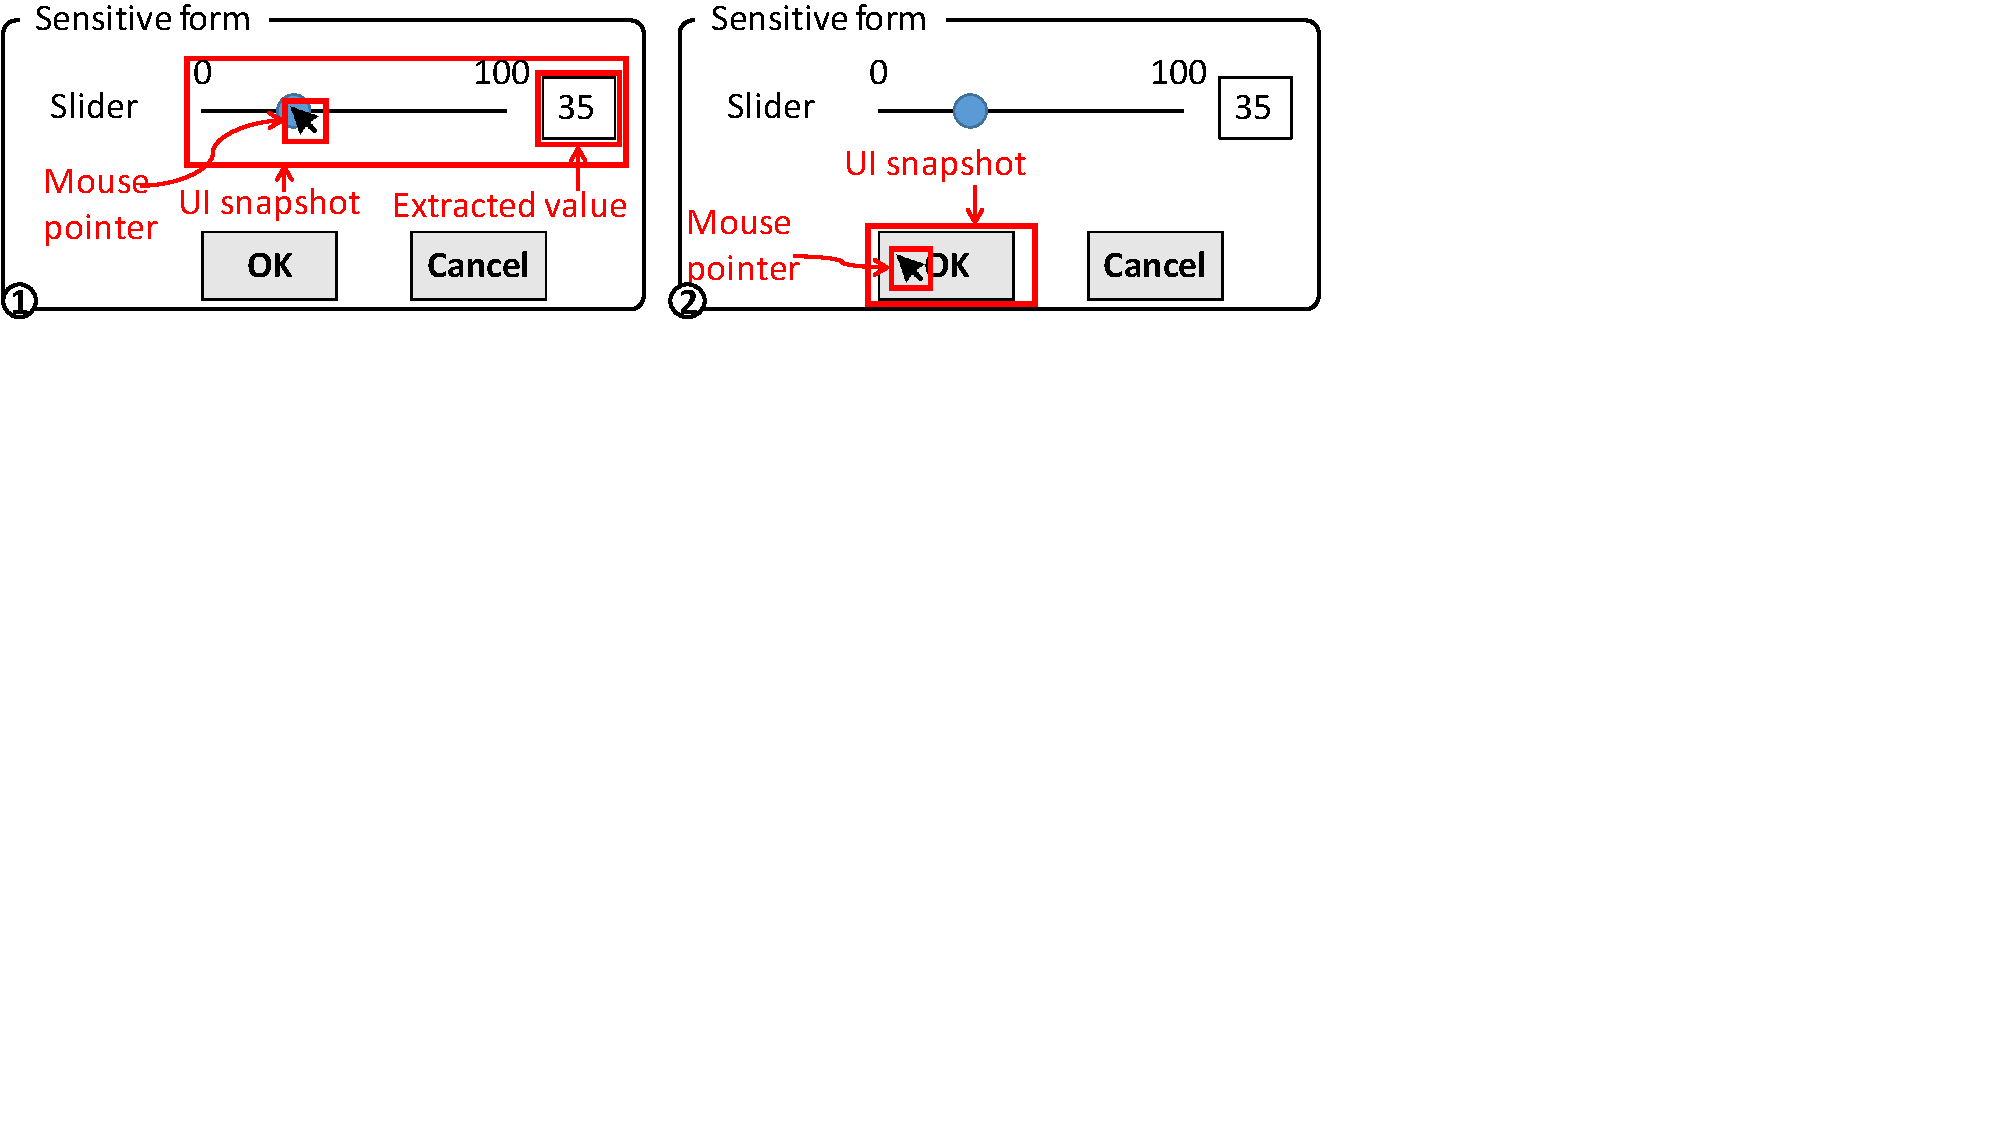
\includegraphics[trim={0 13.5cm 11.5cm 0}, clip, width=\linewidth]{uiDetect_2.pdf}
\caption{\textbf{Strawman solution: Text/Image Analysis of the UIs}. This strawman solution uses image/text analysis to detect the UI element leveraging edge detection and optical character recognition (to extract the labels on the UI element). The solution suffers from lack of robustness where the \device sometime fails to correctly classify the UI elements/labels due to mouse position or colors.}
\label{fig:uiDetect}
\centering
\end{figure}

This strawman solution augments the previous by adding the information that the user sees on the display to prevent UI manipulation attack. As previous, the external trusted device sits between all the IO devices and the host. This enables the device to intercept the HDMI interface. As soon as the user executes an action, e.g., clicking the mouse, the device takes a snapshot of the screen, signs the snapshot and it to the server along with the signed input. The signed snapshot the device could reveal if the untrusted host manipulates the UI.

On the remote server's side, the server uses image/text analysis to extract the information from the UI elements. Such as the label on a button or the markers on a slider, etc. In Figure~\ref{fig:uiDetect} we illustrate an example scenario. This involves the \device to take a screen-shot from the HDMI frame and use image analysis to understand user action. E.g., in Figure~\ref{fig:uiDetect}, \one the user first drags along the slider UI to set a value (\texttt{35}) and then \two the user clicks on the \texttt{OK}. The \device uses character recognition technique to extract the label and the data from the UI. This example shows the apparent complexity of this mechanism that does not scale with all UI. Further investigation and prototype implementation shows several drawbacks of this solution:


\begin{mylist}
  \item \textbf{Incomplete user context.} The proposed method failed to capture the complete context of the user input. Capturing the UI element only around the mouse pointer ignore the input values that are provided by the user. For example, the use may press \texttt{OK} button after providing the sensitive data, but to capture those data, the \device needs to capture more screen area. Such a method would complicate the entire process and does not generalize.
  \item \textbf{Robustness.} Previous research works such as as~\cite{lukaSpoof,Chen:2010:DVS:1754393.1754394} propose detection of a phishing attack by visually analyzing the web interface of the mobile applications. All of these proposed methods fail to achieve 100\% accuracy in the real world scenarios. Our prototype implementation also confirm that the method lacks robustness in real life as most of the time the \device fails to either recognize the UI elements or extract the label from the UI elements properly despite of using state-of-the-art image/text analysis tools~\cite{opencv}. More importantly, adversarial machine learning techniques~\cite{eykholt2017robust,sitawarin2018rogue} could make the image/text recgnition technique insecure.
  \item \textbf{Performance.} The image/text analysis is CPU intensive and causes a low number of frame output by the \device. Commonly used image analysis frameworks such as OpenCV~\cite{opencv} is CPU intensive and it hard to achieve $24$ fps after the operation on the \device that is implemented on an ARM-based Raspberry Pi.
  \item \textbf{TCB.} The image/text analysis functions are needed to be implemented either on the \device or the remote server. Such increases the size of the TCB significantly.
  \item \textbf{Privacy.} Taking the screenshot also reveal other applications that the user is operating which can be a threat to privacy.
\end{mylist}

Due to such limitations, and the inherent offline nature of this solution, we developed more efficient solution to preserve the integrity of user actions on a UI element. We describe the method in the following section. The solution has a trade-off that the developers need to incorporate some small changes to the remote server but provides better security and usability. We describe our solution in the following section.


\subsection{Challenges}


Modern user interfaces (UIs) are diverse and hard to generalize, resulting in many possible ways to provide input and receiving output.  This makes the protection of IO integrity, and confidentiality is a particularly challenging task. For example, given a mouse movement and clicking on a button from the user, it is necessary to understand the user intention that corresponds to the mouse movements. 


The second challenge arises while ensuring IO confidentiality. For mouse input, hiding the mouse movement while keeping all the regular functionality intact is a challenging task as we do not consider large TCB-based solution such as a trusted hypervisor.


Apart from these functional challenges for implementation, there exist multiple attack vectors that we want to provide protection. 


\subsection{High-level Description of the System}

\begin{figure}[t]
\centering
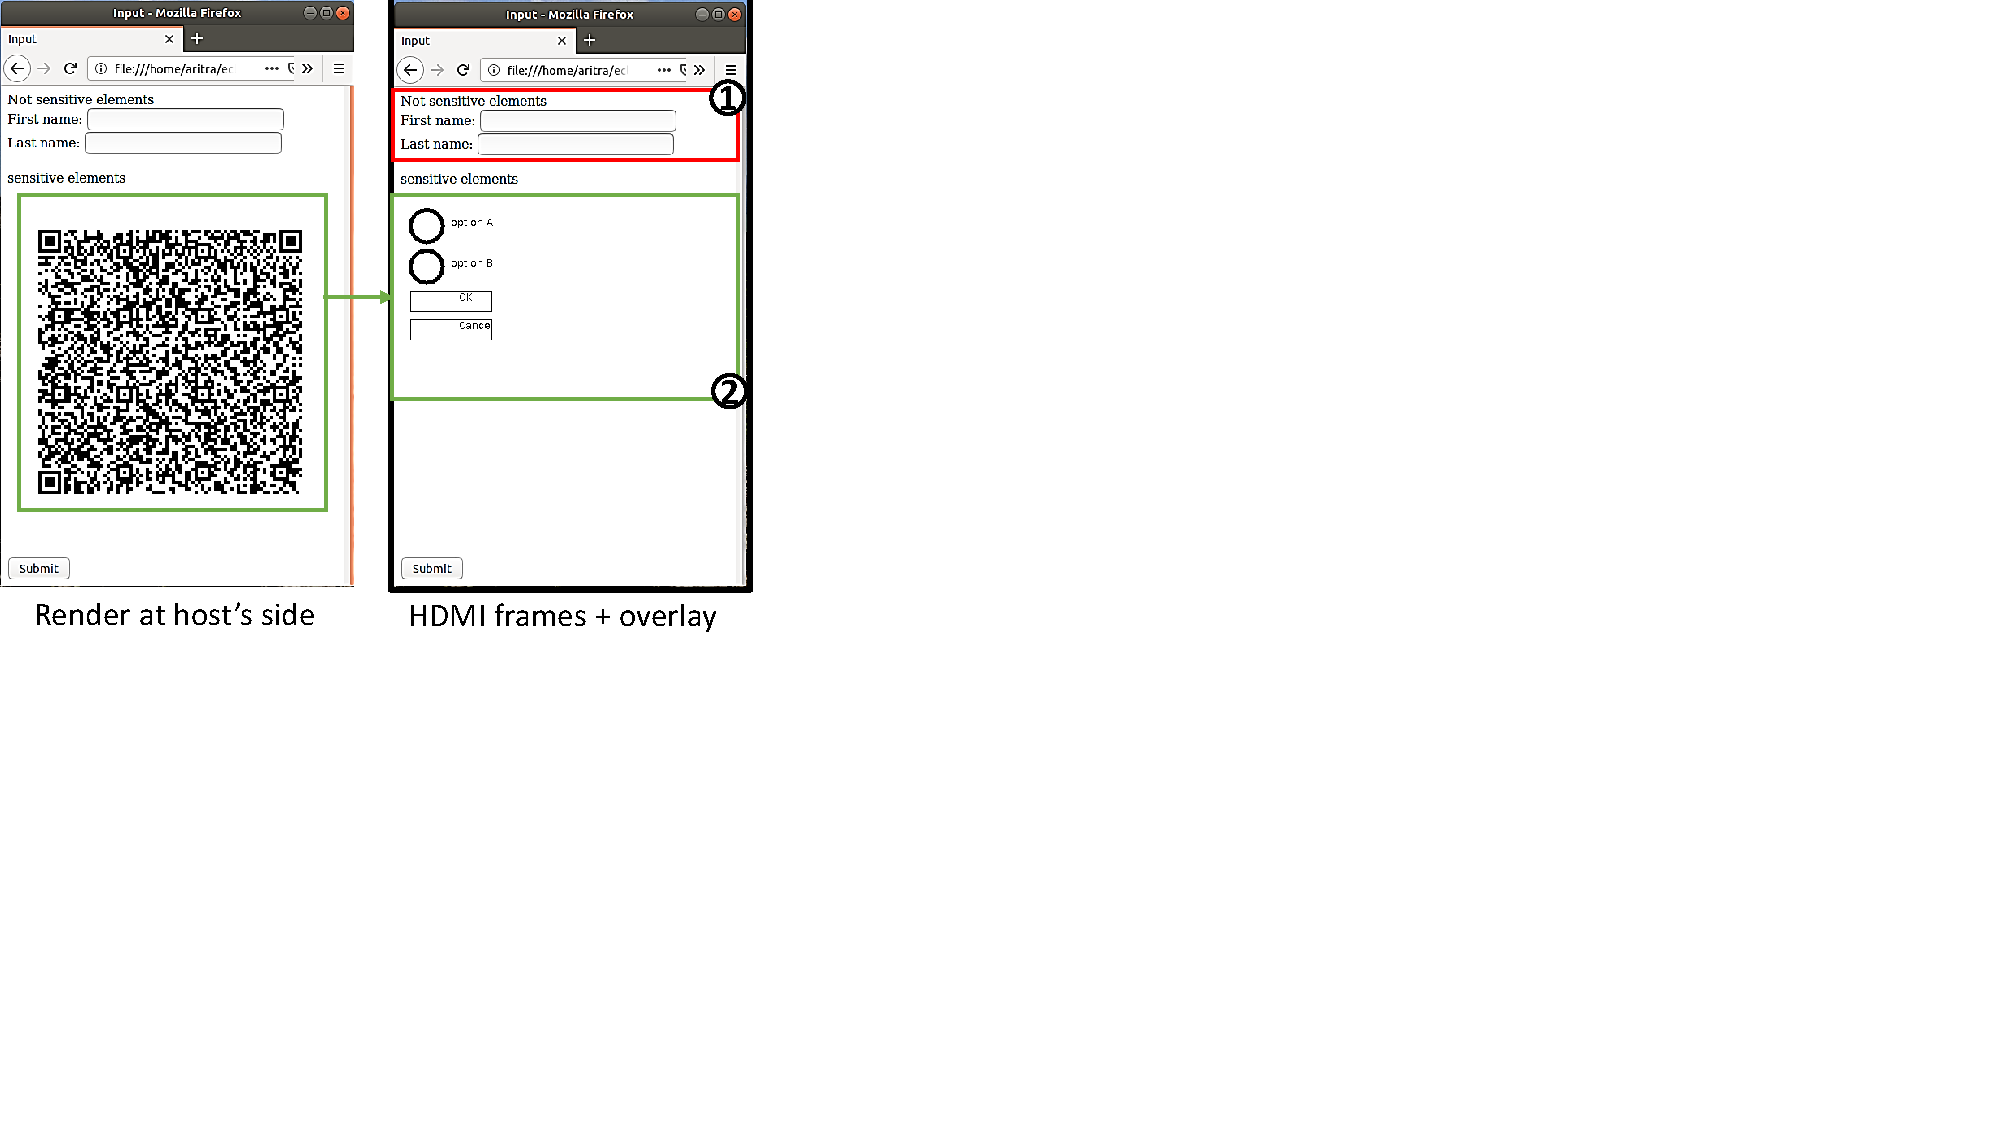
\includegraphics[trim={0 8cm 20cm 0}, clip, width=0.9\linewidth]{overlayScreenShot.pdf}
\caption{\textbf{\device generated UI overlay} The figure shows the \name high-level approach. \one shows the non-protected part of the screen where the Ui is rendered by the untrusted host. \two shows the \device generated protected UI overlay that is hidden from the host. The protected part of the screen provides integrity and confidentiality of all user IO.}
\spacesave
\label{fig:screenshot_1}
\end{figure}

%\myparagraph{Components} \name assumes that IO devices (mouse, keyboard, and display) are connected to a trusted component called \device. This setup allows the trusted \device to receive raw inputs from the user and show overlays on display. The goal of \name is to keep the code running on the \device minimal and at the same time support a wide variety of applications. Thus, we avoid running any application, such as browsers, on the trusted component to keep the TCB very small.

\myparagraph{Key idea} %\red{The key idea of \name is to introduce \emph{root-of-trust} for the IO devices that provides trusted path to remote servers. This is achieved by the \device that provide proof for integrity and confidentiality for all user IO. Thus making the IO devices trustworthy to the users. }
The overall approach is illustrated in Figure~\ref{fig:approachOverview}. On a high level, the remote server and the \device establishes a secure channel using the untrusted host as a transport. Note that the \device does not have any network capabilities, instead uses the host as an untrusted transport.
The \device operates in two modes: passive and active. In the passive mode, the \device serves as a relaying device that forwards mouse and keyboard inputs to the host. Similarly, the \device relays the HDMI frames from the host to the display. Hence, the user experience is not affected when interacting with regular applications. On the active mode, \device has two functionalities: i) intercepts the inputs generated by the user, and ii) render overlays on the HDMI frame that is displayed on the screen. 
The first functionality guarantees that the user inputs arrive directly to a trusted component (\device); therefore, the compromised host cannot manipulate them. The second functionality allows the \device to show trusted information on the screen such as input elements, or data sent from the remote server. A naive solution would be running an entire OS and browser from the \device that provides isolation from the attacker-controlled host. Such approach makes the size of the \device TCB massive, making it to be as vulnerable as the host. 

During the initialization phase, the \device and the remote server share a key that is used to encrypt/sign the communication between each other. The remote server signs the sensitive elements that should be protected and delivers them to the untrusted host. The application running on the host encodes the sensitive elements into the HDMI frame. The \device captures the frames, decodes the sensitive elements, verifies their signatures, and then renders elements into an overlay. Figure~\ref{fig:screenshot_1} provides a screenshot of attacker's view of the screen and the user's view after the \device overlays the UI. \one shows non-sensitive elements that are unprotected, while \two are the protected elements that are not rendered by the untrusted host. In this way, the device guarantees that the user is presented with the legitimate elements sent by the remote server and the user interaction with these elements is managed only by the device itself. Note that the device renders only the protected input elements, while other UI components of the application are rendered by the host. 
Therefore, user inputs (mouse events and keystrokes) addressed to the protected elements are intercepted by the \device and not forwarded to the untrusted host. Furthermore, the \device renders on runtime the user inputs into the overlay while the host is oblivious about them. From the user's perspective, the workflow of filling a form with protected elements remains the same as filling forms of existing applications.

